\chapter{Design and Methodology}\label{chap:Methods }
% =============================================================================
\section{Visualization and User Interface}
% =============================================================================
Scholar Plot obtains the Impact Factor ($IF$) for a particular journal from our database. The data of Impact Factor is acquired from The Thomson Reuters Impact Factor - Web of Science. Based on all this information it constructs the plots as per the design outlined in the Visualization and User Interface section, using nvd3 library \cite{nvd3org}.


The NSF/NIH/NASA funding datasets are available at the respective US government websites in various file formats such as XML, CSV and so on \cite{nsf, nih}. We implemented a script to parse this massive XML dataset into our data structure that consists of AwardID, AwardAmount, First name, Last name, Investigator by RoleCode (Principal Investigator, Co-Principal Investigator and Former Principal Investigator), using XMLStarlet \cite{XMLStarlet}. We imported this data to our database using Toad DBMS tool. %We designed our relational database schema in MySQL.

\begin{figure}%[!htb]
\centering
  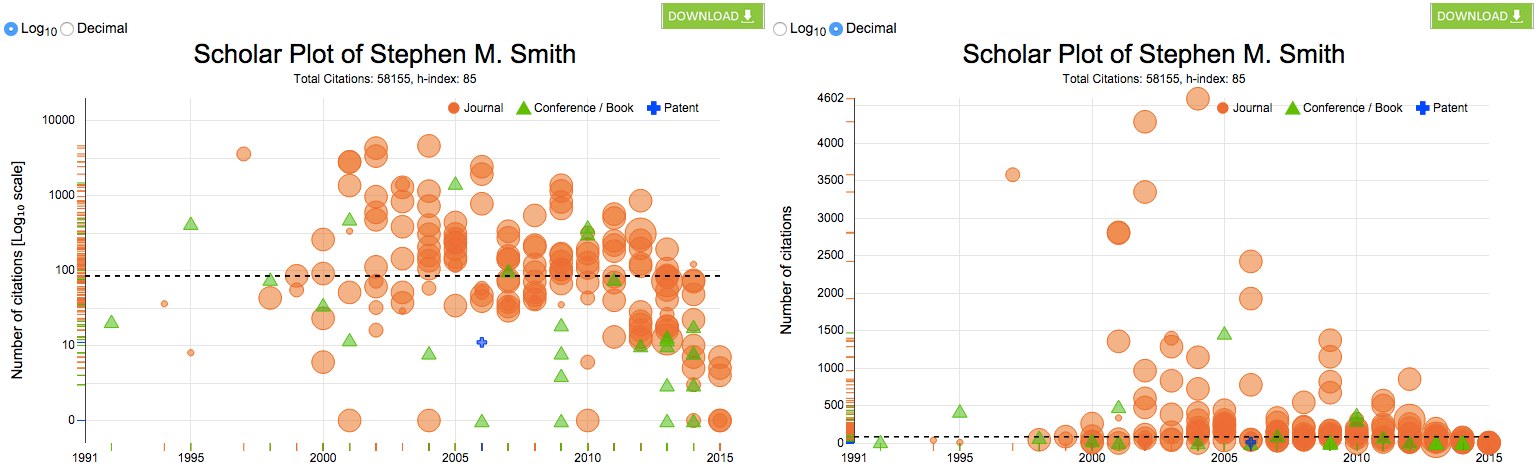
\includegraphics[width=1\columnwidth]{figures/fig_scaleView}
  \caption{The $log_{10}$ view and $decimal$ view: The radio button allows to switch between different scale views without reloading the entire page.}~\label{fig:fig-scale}
\end{figure}

\begin{figure*}
  \centering
  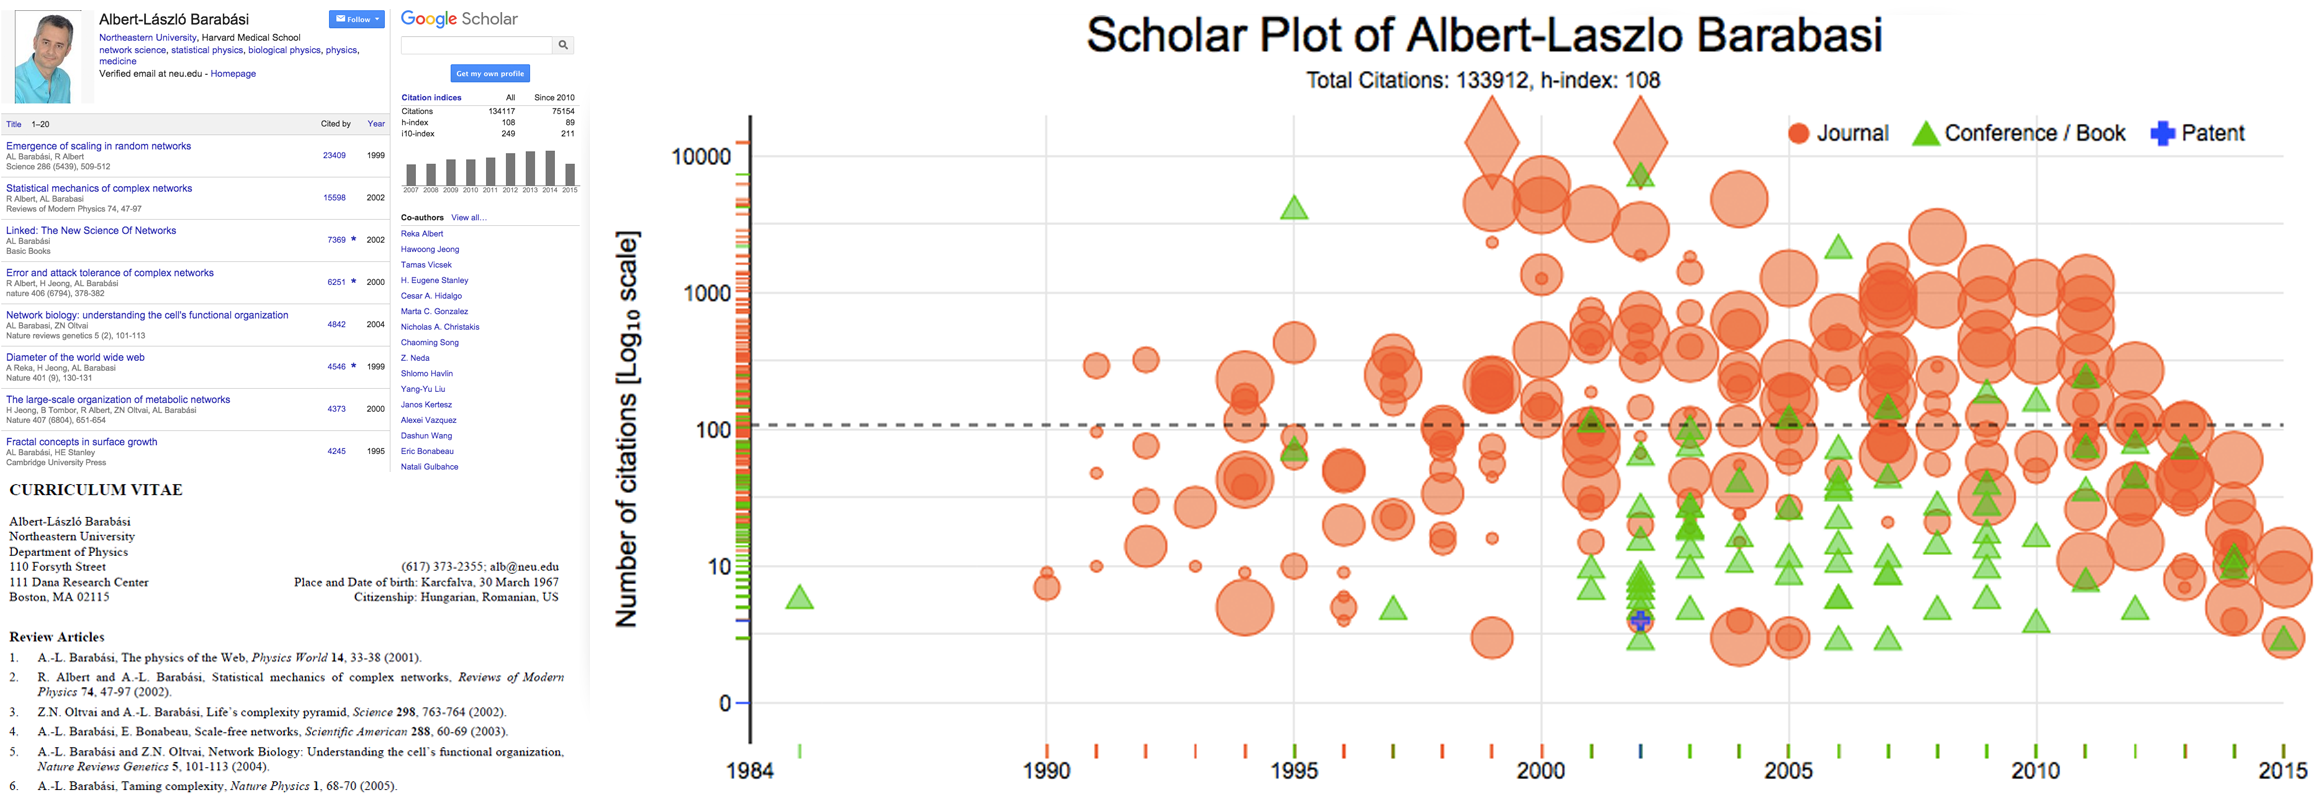
\includegraphics[width=1\columnwidth]{figures/fig_cv_google_scholarplot}
  \caption{An example of Scholar Plot - Visualizing Publication Data}~\label{fig:fig-publication}
 % \vspace{-1ex} 
\end{figure*}

Scholar Plot depicts the publications of an individual as a scatter plot and the NSF/NIH/NASA funding as a multiline plot. The publications are represented in a 2D diagram (number of citations vs. year of publication) with the {\it h}-index line (Figure \ref{fig:fig-publication}). The horizontal axis is time, starting with the year of the researcher's first publication ending with the current year. The vertical axis is the number of citations. The default plot is in $log_{10}$ scale. The user can also view the plot in the decimal scale by a toggle option using a radio button at the top left corner (Figure \ref{fig:fig-scale}). The log scale provides a standardized scale which helps to compare the plots of multiple scholars.



% --------------------------
\subsection{Visualizing Publication Data}
% --------------------------
Each publication $i$ is represented with a symbol. The center of the symbol has coordinates $(i_{PY}, i_{C})$, where $PY$ stands for Publication Year and $C$ for Number of citations obtained by the publication till date. The journals are represented as circles (orange) with area analogous to the impact factor the journal. The conferences / books are represented as triangles (green) and the patents as crosses (blue). By clicking at a symbol you can obtain the publication title, the year, the number of citations, the venue where published and its impact factor (if it is a journal), as well as a breakdown in the authorship, complete with the level of collaboration between the co-authors and the selected scholar (Figure \ref{fig:fig-tooltip}). The publication title also enables the user to navigate to the Google Scholar page for the selected paper. This helps to quickly verify and obtain further details of the selected publication. It makes user reach out to the PDF file directly if available. To enhance user experience, we customized the tooltip to give detailed information without overlapping the plots.

\begin{figure}[H]
\centering
  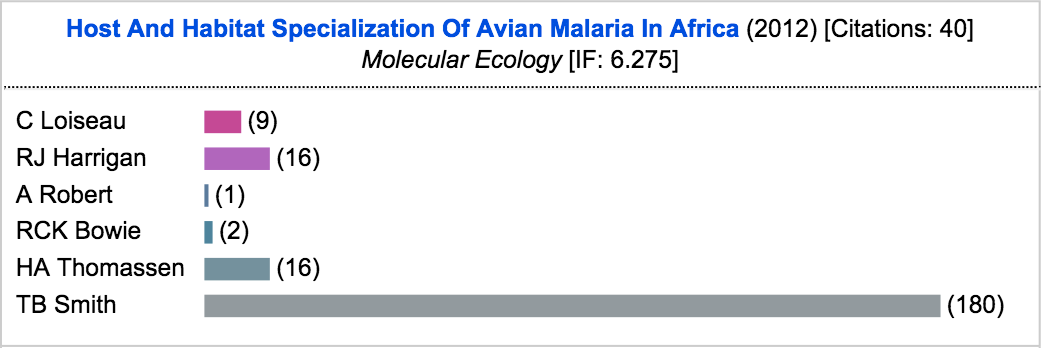
\includegraphics[width=1\columnwidth]{figures/fig_tooltip}
  \caption{An example of the tooltip: The publication title, the year, the number of citations, the venue where published, impact factor, the list of co-authors, the visual horizontal bars with the number of collaboration between the co-authors and the selected scholar.}~\label{fig:fig-tooltip}
 % \vspace{-1ex} 
\end{figure}

A dotted horizontal line on the plot denote the {\it h}-index of the scholar. We also denote those publications which earn greater than 10,000 citations with diamonds as they represent the great success in publications (Figure \ref{fig:fig-publication}). The title of the plot contains the name of the scholar and her/his total number of citations along with the {\it h}-index. At the top right corner of the plot, a legend shows the three different types of publications we distinctly display (Figure \ref{fig:fig-legend}).

\begin{figure}[!htb]
\centering
  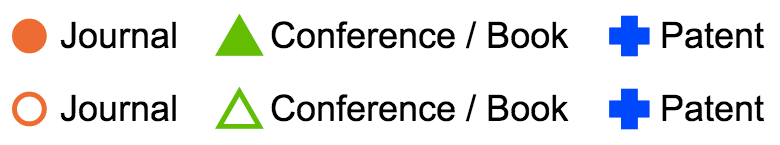
\includegraphics[width=0.9\columnwidth]{figures/fig_legend-toggle}
  \caption{The legend allows users to selectively view journals, conferences / books and patents.}~\label{fig:fig-legend}
 % \vspace{-1ex} 
\end{figure}

You can bring the journals, patents, and conferences / books in and out of the view by clicking at the respective legend. If there is an overlap between journals, conferences and patents, this feature can help the user to selectively view them. The user can also zoom into the plot for closer picture. Also note that the symbols are not completely opaque. So if there are multiple symbols which overlap, the user can see and interact with them by hovering the mouse over them appropriately.

% --------------------------
\subsection{Visualizing Funding Data}
% --------------------------
Scholar Plot also depicts the NSF/NIH/NASA funding of an individual as a multiline (Figure \ref{fig:funding}). Each breakpoint in the multiline corresponds to the individual's total amount in all NSF/NIH/NASA awards for the specific year. By pointing at a breakpoint you can obtain the NSF/NIH/NASA awards IDs, award amounts, and investigator's role. The total annual funding information per year is also available by clicking the legend. 

\begin{figure}[!htb]
  \centering
  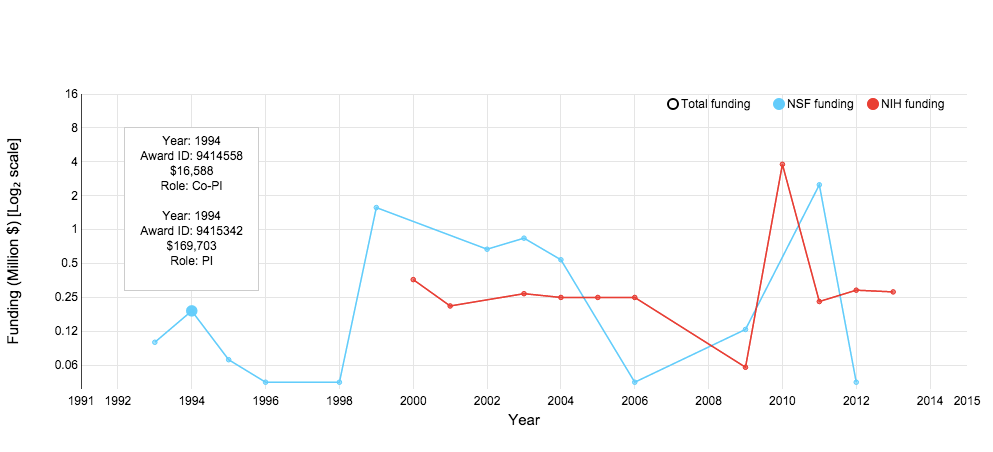
\includegraphics[width=1\columnwidth]{figures/fig_funding_default}
  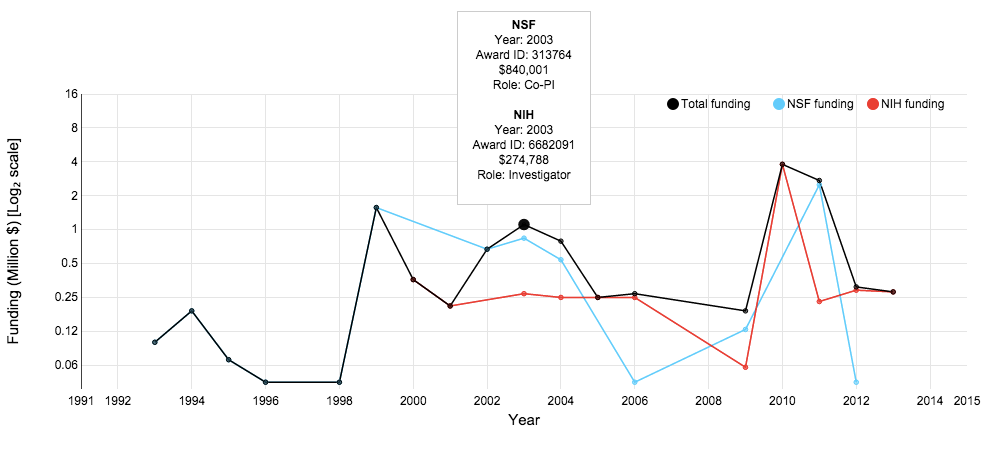
\includegraphics[width=1\columnwidth]{figures/fig_funding_total}
  \caption{An example of Scholar Plot - Visualizing Funding Data}~\label{fig:funding}
  % \vspace{-2ex} 
\end{figure}



%% --------------------------
%\subsection{Disk Size - How to determine the size of disks}
%% --------------------------
%We wanted to plot to visualize more efficiently with different size of disk for Journal publications that tells the different ranking of Journal by Impact Factor Index. To do this, we analyzed the data set of JCR 2013 IF and run quartile function as a useful concept in statistics to determine the size of disks in Scholar Plot. Based on this number, the system will decide the size of plot of each journal data and plot it in real-time. The quartile values are shown in table Table~\ref{tab:table1}. The maximum number from descriptive is 153.459 through. 
%
%\begin{table}
%  \centering
%  \begin{tabular}{c c}
%    \toprule
%    \multicolumn{2}{c}{\small{\textbf{ JCR Data (Impact Factor 2013) }}} \\
% 
%    {\small\textbf{Quartiles}}
%    & {\small \textit{IF}} \\
%    \midrule
%    Q1 & 0.67 \\
%    Q2 & 1.36 \\
%    Q3 & 2.47 \\
%    Q4 & 51.66 \\
%    \bottomrule
%  \end{tabular}
%  \caption{Table captions should be placed below the table. We
%    recommend table lines be 1 point, 25\% black. Minimize use of
%    unnecessary table lines.}~\label{tab:table1}
%\end{table}

%Scholar Plot gives a snapshot of the individuals profile in a concise manner.
To place the plots in your personal CV or on your web page we provide a download button at the top right corner of the plot (Figure \ref{fig:fig-scale}). This function enables the user to download plots in a zip file. It includes high resolution vector images in SVG (Scalable Vector Graphics) format of the publication and funding plots.

Scholar Plot also has a projection of the data on the y-axis depicted by small horizontal colored lines. For example, we can clearly see that journals contribute to the {\it h}-index of scholar in Figure \ref{fig:distribution} (a) and conferences / books contribute to the {\it h}-index of scholar in Figure \ref{fig:distribution} (b). We can clearly infer the scholar in Figure \ref{fig:distribution} (c)) has many patents. We can also infer the number of publications within a particular range of citations based on the density of the projected lines.

\begin{figure}[!htb]
\centering
\subfigure[]{%
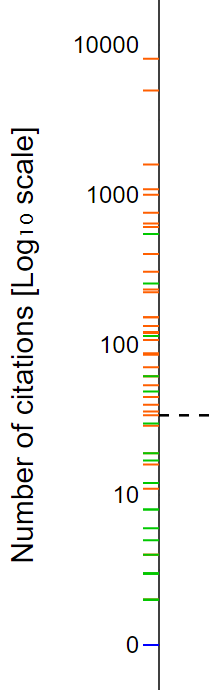
\includegraphics[width=0.23\columnwidth]{figures/fig_distribution_A}
}
\subfigure[]{%
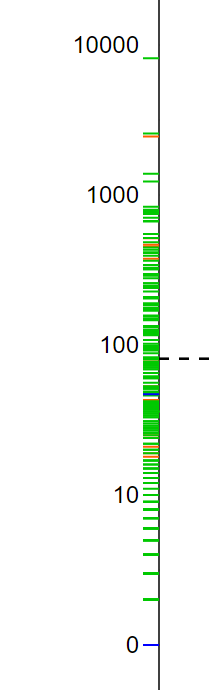
\includegraphics[width=0.23\columnwidth]{figures/fig_distribution_B}
}
\subfigure[]{%
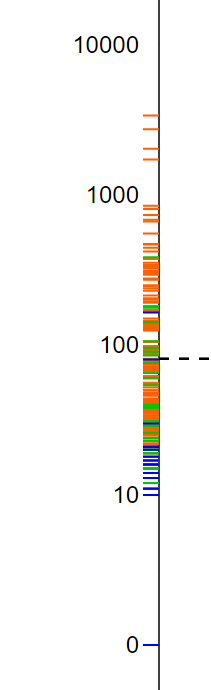
\includegraphics[width=0.23\columnwidth]{figures/fig_distribution_C}
}
\caption{Examples of y-axis projection for three different scholars.}~\label{fig:distribution}
  %\vspace{-1ex} 
\end{figure}

%\begin{figure}[!htb]
%  \centering
%  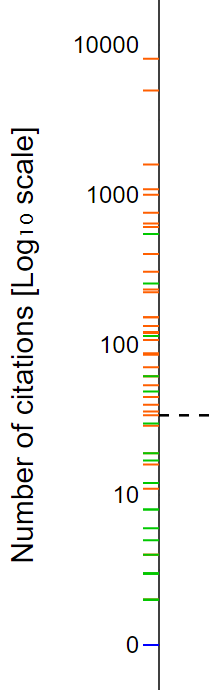
\includegraphics[width=0.2\columnwidth]{figures/fig_distribution_A}
%  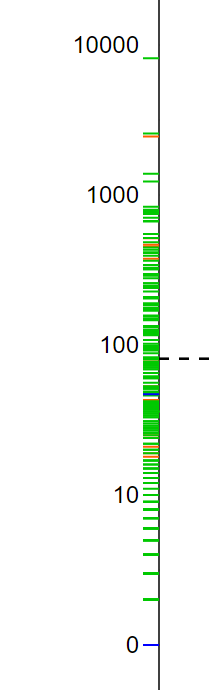
\includegraphics[width=0.2\columnwidth]{figures/fig_distribution_B}
%  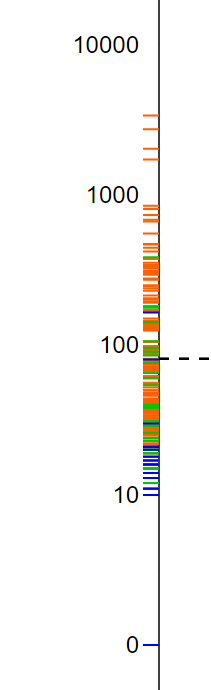
\includegraphics[width=0.2\columnwidth]{figures/fig_distribution_C}
%  \caption{Example with journals, conferences, and patents contributing to h-index}~\label{fig:distribution}
%\end{figure}

We improve user experience to enable users to quickly find and select from a pre-populated list of scholar names as they type. For each character the user enters, we display similar matching names on the dropdown list. Even entering the space (`` "), we display the 10 most recently inserted scholar's names. Scholar Plot follows the approach of responsive web design to provide optimal viewing based on the size of screen.



